\chapter{Sistemi Numerici}
\section{Introduzione}
L'aritmetica svolta dai computer differice dall'aritmetica a noi familiare, i motivi sono molteplici, ma quello prinicipale è sicuramente da attribuire alla diversa modalità neòòa rappresentazione dei dati e delle informazioni.

\begin{align*}
    16_{10} & \neq 16_{16} \quad \text{(16 in decimale è diverso da 16 in esadecimale)} \\[8pt]
    16_{10} &= 1 \cdot 10^1 + 6 \cdot 10^0 = 16_{10} \\
    16_{16} &= 1 \cdot 16^1 + 6 \cdot 16^0 = 22_{10}
\end{align*}

Se per noi il sistema decimale può sembrare scontato, non è certo lo stesso per i computer, infatti, i calcolatori lavorano sfruttando il sistema binario.

\section{Bit}
\subsection{Definizione}
Con il termine \textbf{bit} definiamo l'unità di misura dell'informazione, un bit \uline{può assumere solo il valore di 0 o 1}

\subsection{Unità di misura}
Combinando tra loro più bit si ottengono strutture complesse, in particolare:
\begin{itemize}
    \item Byte - 8 bit
    \item Nybble - 4 bit
    \item Word - 32 bit
    \item Halfword - 16 bit
    \item Doubleword - 64 bit
\end{itemize}

\subsection{Numero di configurazione possibili}
Dati \textbf{k bit} il \uline{numero di configurazione ottenibili è pari a $2^k$}

\newpage
\section{Rappresentazione di un sistema numerico posizionale}
\subsection{Cosa è un sistema numerico posizionale?}
È un sistema numerico dove ogni cifra assume un valore diverso a seconda della posizione che occupa all'interno del numero

\subsection{Formula}
\begin{tcolorbox}
    {
        \LARGE
        $$
            N = \sum^{n-1}_{i=-m} d_i \cdot r^i
        $$
    }
    \begin{itemize}
        \item[$d$ -] rappresenta la singola cifra
        \item [$r$ -] è la radice o base del sistema
        \item [$n$ -] è il numero di cifre della parte intera (sinistra della virgola)
        \item [$m$ -] è il numero di cifre della parte frazionaria (destra della virgola)
    \end{itemize}
    
    \subsubsection{Esempio d'uso formula}
    {
        \Large
        \begin{gather*}
            15 = 10 \cdot 10^1 + 5 \cdot 10^0
        \end{gather*}
    }
\end{tcolorbox}

\section{Sistema Binario}
\subsection{Definizione}
\begin{itemize}
    \item Base: $r=2$
    \item Cifre: $d=0,1$
    \item Un valore numerico $N$ si rappresenta come:
    {\large
        $$
            N = d_{n-1} \cdot 2^{n-1} + \dots + d_0 \cdot 2^0 + d_{-1} \cdot 2^{-1} + \dots + d_{-m} \cdot 2^{-m}
        $$
    }
\end{itemize}

\subsection{Esempio}
{
    \Large
    $$
        101_2 = 1 \cdot 2^2 + 0 \cdot 2^1 + 1 \cdot 2^0 = 5_{10}
    $$
}

\subsection{Byte}
È una sequenza di otto bit consecutivi

\begin{center}
    \begin{minipage}{0.3\textwidth}
        \begin{center}
            
            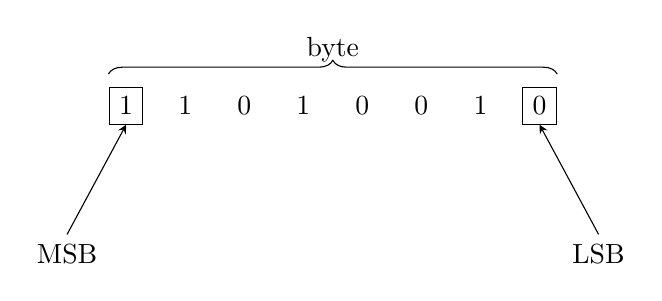
\begin{tikzpicture}[x=0.5cm, y=0.5cm, >=stealth, scale=1.5]
            
                % 1. BIT INDIVIDUALI (Garantisce allineamento perfetto)
                \node (b7) at (0,0) {1};
                \node (b6) at (1,0) {1};
                \node (b5) at (2,0) {0};
                \node (b4) at (3,0) {1};
                \node (b3) at (4,0) {0};
                \node (b2) at (5,0) {0};
                \node (b1) at (6,0) {1};
                \node (b0) at (7,0) {0};
            
                % 2. REPTANGOLI SU MSB (b7) E LSB (b0)
                \draw (b7.south west) rectangle (b7.north east);
                \draw (b0.south west) rectangle (b0.north east);
            
                % 3. GRAFFA SUPERIORE
                \draw[decorate, decoration={brace, amplitude=5pt, raise=3pt}] 
                    (-0.3, 0.4) -- (7.3, 0.4) 
                    node[midway, yshift=12pt] {byte};
            
                % 4. TESTI MSB / LSB
                \node (msb) at (-1, -2.5) {MSB};
                \node (lsb) at (8, -2.5) {LSB};
            
                % 5. FRECCE
                \draw[->] (msb.north) -- (b7.south);
                \draw[->] (lsb.north) -- (b0.south);
            
            \end{tikzpicture}
        \end{center}
    \end{minipage}
    \hfil
    \begin{minipage}{0.33\textwidth}
        \begin{itemize}
            \item Most Significant Bit (MSB): il bit più a sinistra \\
            \item Least Significant Bit (LSB): il bit più a destra
        \end{itemize}
    \end{minipage}
\end{center}

\section{Sistema Ottale}
\subsection{Definizione}
\begin{itemize}
    \item Base $r=8$
    \item Cifre $d=0,1,\dots,7$
    \item Un valore numerico $N$ si rappresenta come:
    {\large
        $$
            N = d_{n-1} \cdot 8^{n-1} + \dots + d_0 \cdot 8^0 + d_{-1} \cdot 8^{-1} + \dots + d_{-m} \cdot 8^{-m}
        $$
    }
\end{itemize}

\subsection{Esempio}
{
    \Large
    $$
        127_8 = 1 \cdot 8^2 + 2 \cdot 8^1 + 7 \cdot 8^0 = 87_{10}
    $$
}
